\documentclass{beamer}
\usepackage[utf8]{inputenc}
%\usepackage[margin=1in]{geometry}
\usepackage{tikz}
\usetikzlibrary{patterns,intersections,angles,quotes, calc, graphs, positioning}
\usepackage{array}
\usepackage{graphicx}
\usepackage{lmodern}
\usepackage{amsmath,amsthm,amssymb}
\usepackage[italic]{esdiff}
\usepackage{mathtools}
\usepackage{fancyhdr}
\usepackage{listings}
\lstset{numbers=left, numberstyle=\tiny, stepnumber=1,firstnumber=1,
    numbersep=5pt,language=Python,
    stringstyle=\ttfamily,
    basicstyle=\footnotesize, 
    showstringspaces=false
}
\AtBeginSection[]{
  \begin{frame}
  \vfill
  \centering
  \begin{beamercolorbox}[sep=8pt,center,shadow=true,rounded=true]{title}
    \usebeamerfont{title}\insertsectionhead\par%
    \vspace{1cm}
  \end{beamercolorbox}
  { 
          \begin{minipage}{4cm}
              \begin{center}
                 \small \tableofcontents[currentsection]
              \end{center}
          \end{minipage}
  }
  \vfill
  \end{frame}
}

\usepackage{color}

\definecolor{mygreen}{rgb}{0,0.6,0}
\definecolor{mygray}{rgb}{0.5,0.5,0.5}
\definecolor{mymauve}{rgb}{0.58,0,0.82}

\lstset{ 
  backgroundcolor=\color{white},   % choose the background color; you must add \usepackage{color} or \usepackage{xcolor}; should come as last argument
  basicstyle=\footnotesize\ttfamily,        % the size of the fonts that are used for the code
  breakatwhitespace=false,         % sets if automatic breaks should only happen at whitespace
  breaklines=true,                 % sets automatic line breaking
  captionpos=b,                    % sets the caption-position to bottom
  commentstyle=\color{mygreen},    % comment style
  deletekeywords={...},            % if you want to delete keywords from the given language
  escapeinside={\%*}{*)},          % if you want to add LaTeX within your code
  extendedchars=true,              % lets you use non-ASCII characters; for 8-bits encodings only, does not work with UTF-8
  frame=single,	                   % adds a frame around the code
  keepspaces=true,                 % keeps spaces in text, useful for keeping indentation of code (possibly needs columns=flexible)
  keywordstyle=\color{blue},       % keyword style
  language=Octave,                 % the language of the code
  morekeywords={*,...},            % if you want to add more keywords to the set
  numbers=left,                    % where to put the line-numbers; possible values are (none, left, right)
  numbersep=5pt,                   % how far the line-numbers are from the code
  numberstyle=\tiny\color{mygray}, % the style that is used for the line-numbers
  rulecolor=\color{black},         % if not set, the frame-color may be changed on line-breaks within not-black text (e.g. comments (green here))
  showspaces=false,                % show spaces everywhere adding particular underscores; it overrides 'showstringspaces'
  showstringspaces=false,          % underline spaces within strings only
  showtabs=false,                  % show tabs within strings adding particular underscores
  stringstyle=\color{mymauve},     % string literal style
  tabsize=2,	                   % sets default tabsize to 2 spaces
  title=\lstname                   % show the filename of files included with \lstinputlisting; also try caption instead of title
}
\usepackage{hyperref}
\setbeamercovered{invisible}
\setbeamercovered{%
again covered={\opaqueness<1->{15}}}
\title{Current State of Zooniverse Jets}
\author{Charlie Kapsiak}

\begin{document}

\frame{\titlepage}

\begin{frame}{Where is it?}
    All work can be found in the github repository: \url{https://github.com/CharKap/Solar_Zooniverse_Processor}.
\end{frame}

\begin{frame}
    \frametitle{Topics}
    \begin{itemize}[<+->]
        \item Preprocessor finished
        \item Documentation mostly finished
        \item Zooniverse page mostly finished
    \end{itemize}
\end{frame}

\section{Image Preprocessing}%

\begin{frame}{Package Capabilities}
    \begin{itemize}
        \item    Interface with external services like HEK
        \item    Store persistent information to avoid redundant calls to the services
        \item    Generate visuals based on information acquired from these services
        \item    Export visuals and data in a format compatible with Zooniverse
        \item    Import data from zooniverse as usable python objects
        \item    Aggregate the imported data
    \end{itemize} 
\end{frame}

\begin{frame}[fragile]
    \begin{figure}

        \scalebox{0.7}{
    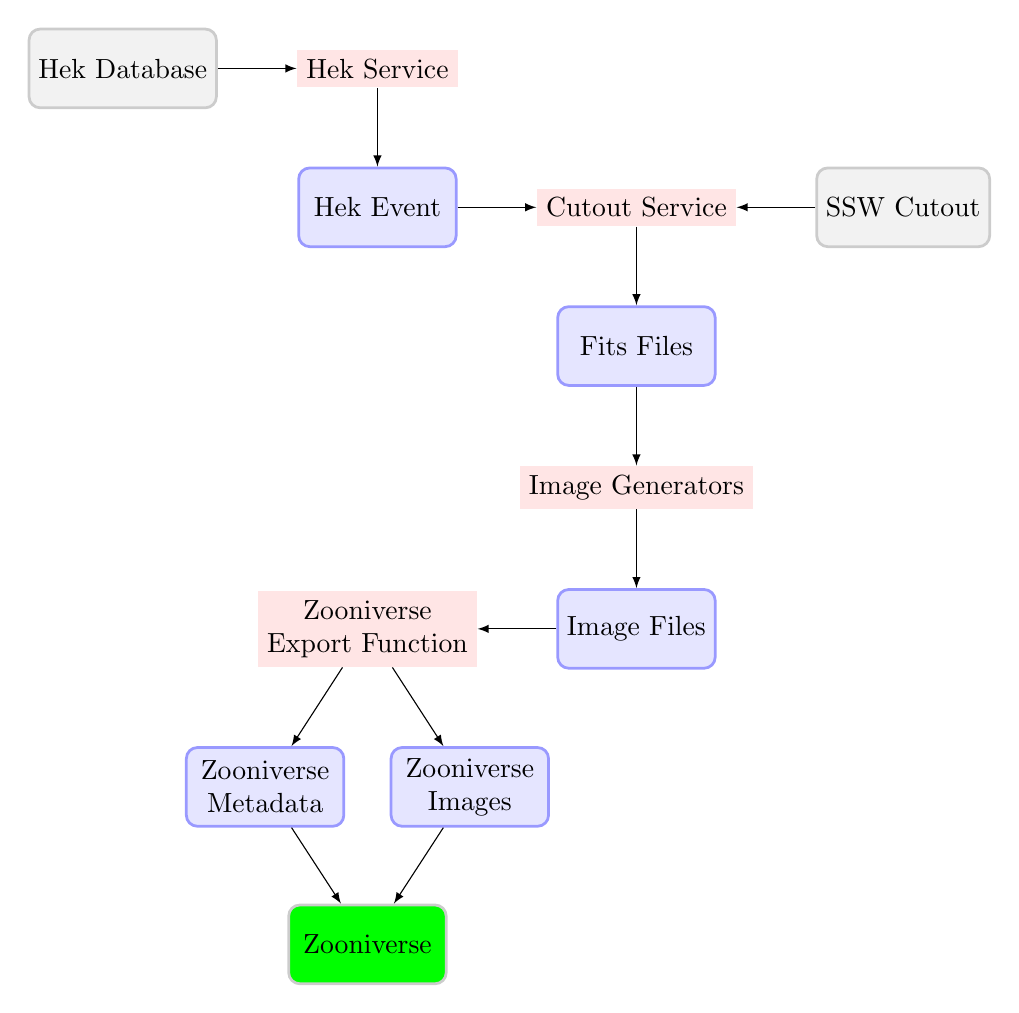
\begin{tikzpicture}[node distance = 1cm]
        \def\colorext{gray}
        \def\colordata{blue}
        \def\colorclass{red}
        \tikzset{shiftnode/.style = {yshift=-1cm}}
        \tikzset{external/.style={draw,
                align=center,
                line width = 1, 
                fill= \colorext!10, 
                draw = \colorext!40, 
                minimum width = 2cm,
                minimum height = 1cm,
                rounded corners
        }}
        \tikzset{database/.style={draw,
                align=center,
                line width = 1, 
                fill= \colordata!10, 
                draw = \colordata!40, 
                minimum width = 2cm,
                minimum height = 1cm,
                rounded corners
        }}
        \tikzset{fetcher/.style={
                align=center,
                in front of path,
                fill=\colorclass!10,
        }}
        \tikzset{connector/.style={-latex}}

        \node[external] (hekdatabase) at (-3,0) {Hek Database};
        \node[fetcher, right=of hekdatabase] (hekserv) {Hek Service};
        \node[database, below=of hekserv] (hekev) {Hek Event};
        \draw[connector] (hekdatabase) -- (hekserv);
        \draw[connector] (hekserv) -- (hekev);
        \node[fetcher, right=of hekev] (cutserv) { Cutout Service};
        \node[external, right=of cutserv] (ssw) {SSW Cutout};
        \draw[connector] (hekev) -- (cutserv);
        \draw[connector] (ssw) -- (cutserv);
        \node[database, below=of cutserv] (fits) {Fits Files};
        \draw[connector] (cutserv) -- (fits);
        \node[fetcher, below=of fits] (imggen) {Image Generators};
        \node[database, below=of imggen] (img) {Image Files};
        \draw[connector] (fits) -- (imggen);
        \draw[connector] (imggen) -- (img);
        \node[fetcher, left = of img] (zoogen) {Zooniverse \\ Export Function};
        \node[database, xshift = 1.3cm , below=of zoogen] (zooimg) {Zooniverse\\ Images};
        \node[database,xshift = -1.3cm, below=of zoogen] (zoometa) {Zooniverse\\ Metadata};
        \draw[connector] (img) -- (zoogen);
        \draw[connector] (zoogen) -- (zooimg);
        \draw[connector] (zoogen) -- (zoometa);

        \node[external, fill=green, below= of zoogen, yshift = -2cm] (zoo) {Zooniverse};
        \draw[connector] (zooimg) -- (zoo);
        \draw[connector] (zoometa) -- (zoo);

      %#  \matrix[draw] at (-3,-4.5) {
      %#      \node[external, minimum size=3mm] {}; & 
      %#          \node[] {External Services}; \\ 
      %#          \node[database, minimum size=3mm] {}; & 
      %#              \node[] {Local Data}; \\ 
      %#              \node[fetcher, minimum size=3mm] {}; & 
      %#                  \node[] {Python Utility classes}; \\ 
      %#                  } ;
                \end{tikzpicture}
}
\end{figure}
\end{frame}

\section{Program Features}

\begin{frame}[fragile]
    \frametitle{Setting up the Database}
    In order to have persistence, we must first create the database. This is done by using the function create\_tables(). \\

    \begin{lstlisting}[language=Python]
import solar.database as db
db.create_tables()
    \end{lstlisting}

\end{frame}

\begin{frame}[fragile]
    \frametitle{Getting Events From HEK}
    Once the database has been setup we can begin to search the hek database for potential events. The interface for the HEK api is provided by the class Hek\_Service. \\

    \begin{lstlisting}[language=Python]
import solar.service.hek as hserv
hek = hserv.Hek_Service(
    event_starttime="2015-10-01T00:00:00",
    event_endtime="2015-11-15T00:00:00",
    event_type=["cj"],
)
hek.submit_request()
found_events = hek.fetch_data()
hek.save_data()
    \end{lstlisting}

\end{frame}


\begin{frame}[fragile]
    \frametitle{Getting Fits Files from the Cutout Service}
There are several ways to generate a new Cutout\_Service. One may use an existing request or create one from attributes.

    \begin{lstlisting}[language=Python]
from solar.database import Hek_Event, Cutout_Service
from solar.service.attribute import Attribute
cutout = Cutout_Service(Attribute("param1", val1), \
        Attribute("param2", val2))
cutout = Cutout_Service(param1 = val1, param2 = val2)
event =  Hek_Event.get()
cutout = Cutout_Service._from_event(event)
old_cutout_request = Service_Request.select().where(
            Service_Request.service_type='ssw'
        ).get()
cutout = Cutout_Service._from_model(old_cutout_request)
cutout.subit_request()
cutout.fetch_data()
cutout.save_data()
cutout.save_request()
    \end{lstlisting}

\end{frame}

\begin{frame}[fragile]
    \frametitle{Generating Visuals}
Visuals can be generated by using the image factories found in the solar.visual.img. Videos can be generated using the factories in solar.visual.vid.

There are two ways to generate visual. If persistence is not required, then the image can be generated using the factory itself.

\begin{lstlisting}[language=Python]
import solar.visual.img as im
image_builder = im.Basic_Image("png")
f = Fits_File.get()
image_builder.create(f.file_path)
image_builder.save_visual(f,"savepath.png")    
\end{lstlisting}
\vspace{-0.8cm}
\begin{lstlisting}[language=Python]
import solar.visual.img as im
from solar.database.tables.visual_file \ 
        import Visual_File
image_builder = im.Basic_Image("png")
f = Fits_File.get()
db_image = Visual_File.create_new_visual(f,image_builder)
\end{lstlisting}
\end{frame}

\begin{frame}[fragile]
    \frametitle{Exporting To Zooniverse}
Once we have a collection of images, we can export them. The function zooniverse\_export() Takes a variable number of lists of lists of visual files and outputs them in a format readable by zooniverse.

The split function is used to break a list into manageable chunks, with overlap.
\begin{lstlisting}[language=Python]
import solar.zooniverse.export as ex
files_per_subject = 10
subject_overlap = 2
v = Visual_File.select().where() # Search is narrowed here
ex.zooniverse_export(split(split(v,files_per_subjet, subject_overlap)))
\end{lstlisting}
\end{frame}


\section{More On Visuals}
\begin{frame}[fragile]
    \frametitle{Annotations}
\begin{onlyenv}<1>
The package includes tools to annotate images. 
    \begin{figure}[htpb]
        \centering
        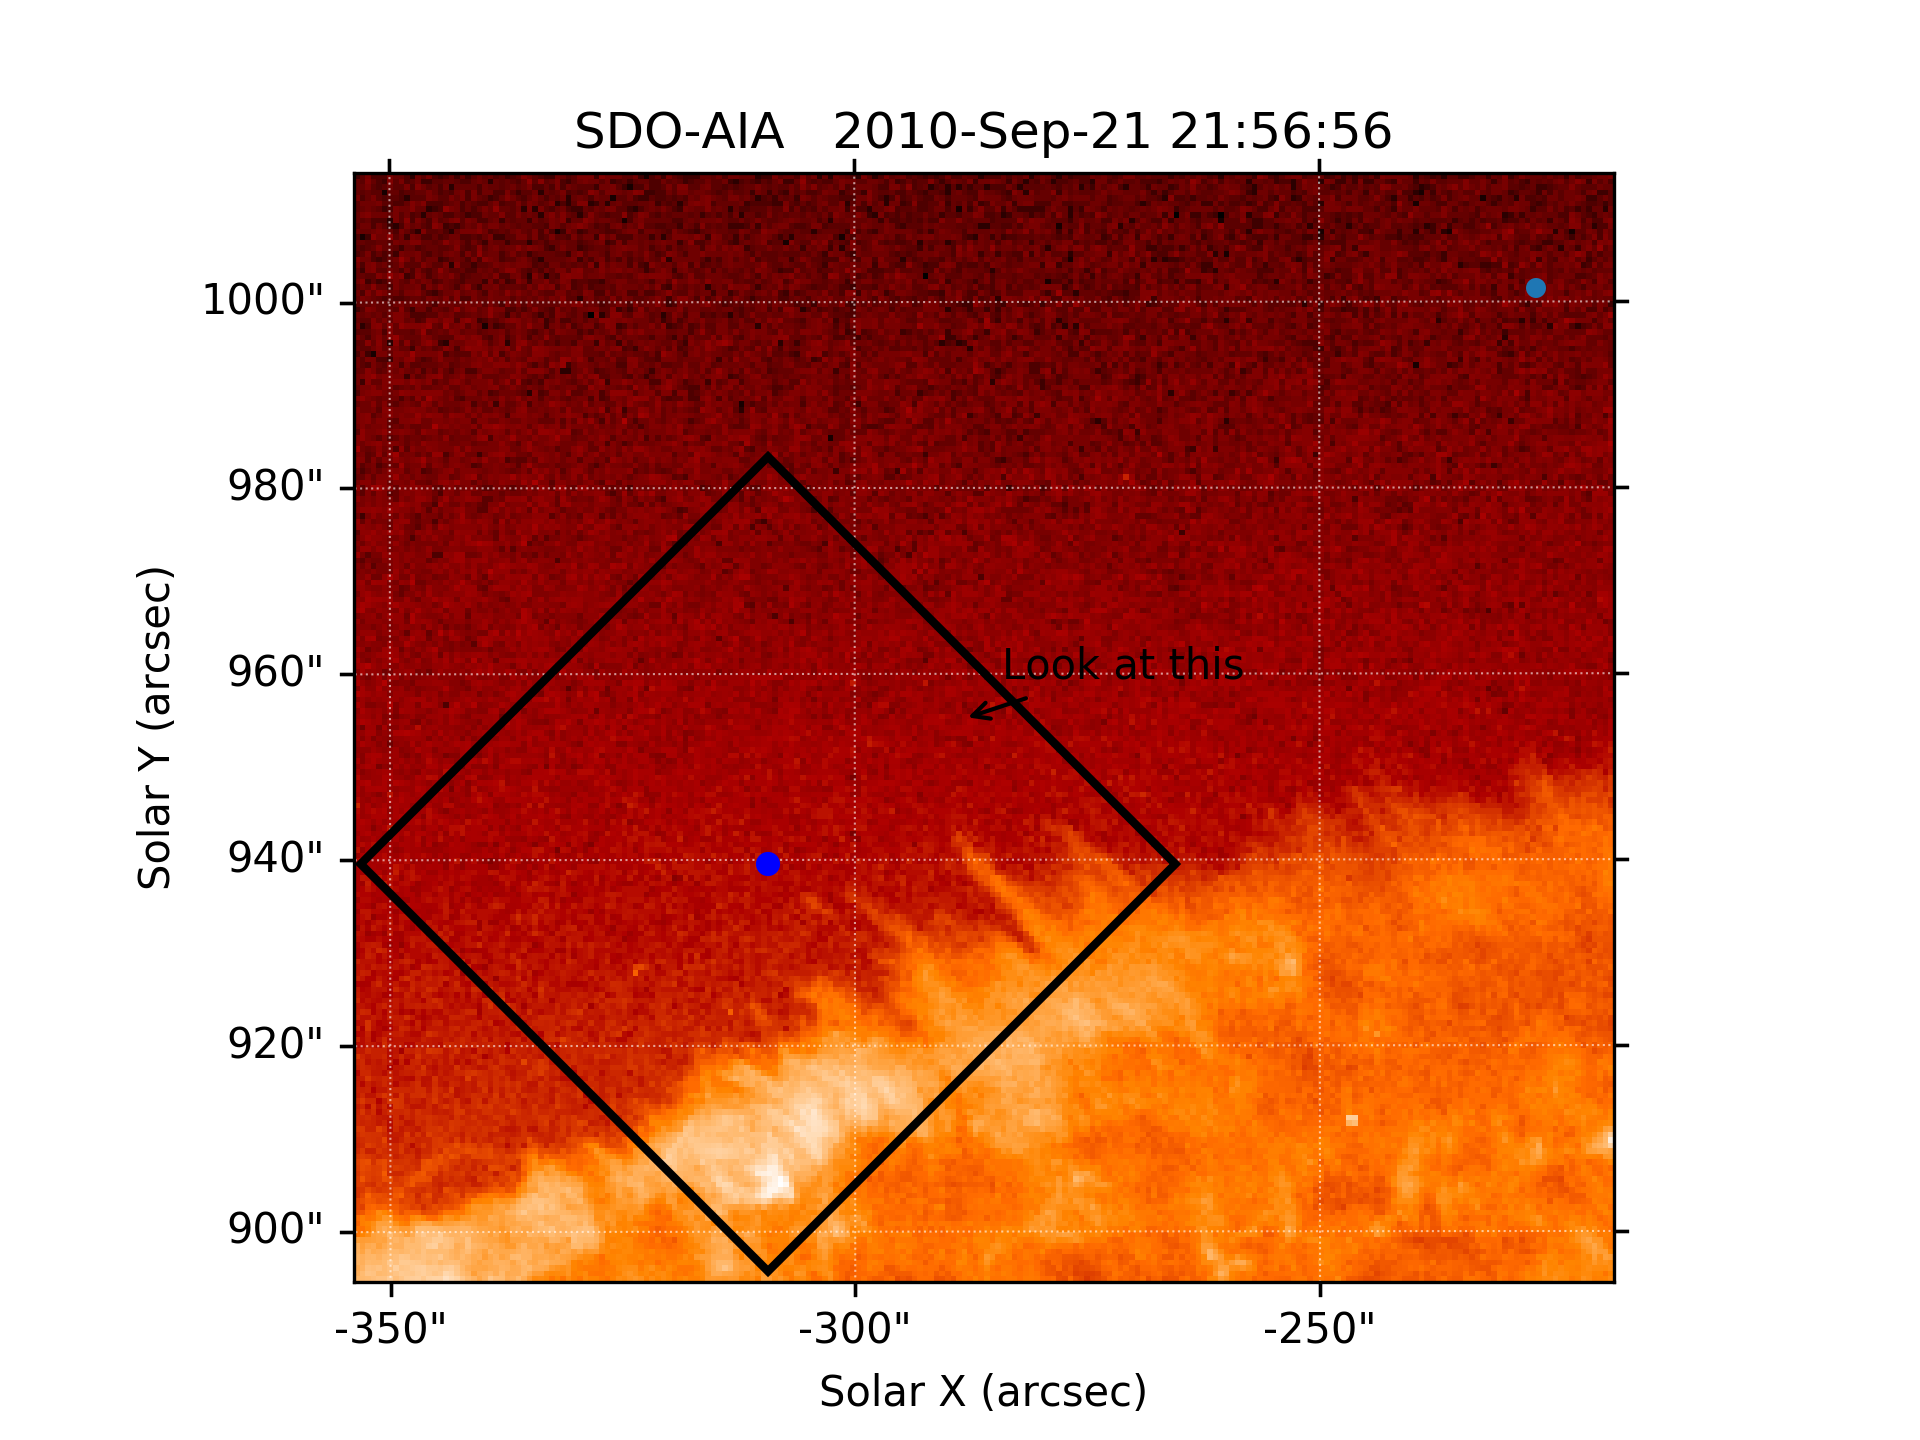
\includegraphics[width=0.8\linewidth]{images/annots.png}
        \caption{images/Annots}%
        \label{fig:images/annots}
\end{figure}
\end{onlyenv}
\begin{onlyenv}<2>
\begin{lstlisting}[language=Python]
rect = Rect_Annot(x=0.4, y=0.4, w=0.3, h=0.4, a=45, lw=2)
circ = Circle_Annot(x=0.8, y=0.8)
rect_center = Circle_Annot(x=0.4, y=0.4, color="blue")
text = Text_Point(0.5, 0.5, "Look at this")
bim.add_annotation(rect, circ, rect_center, text)
fits_database_id = 1
f = Fits_File.get(Fits_File.id == fits_database_id)
bim.create(f.file_path)
\end{lstlisting}
    \begin{figure}[htpb]
        \centering
        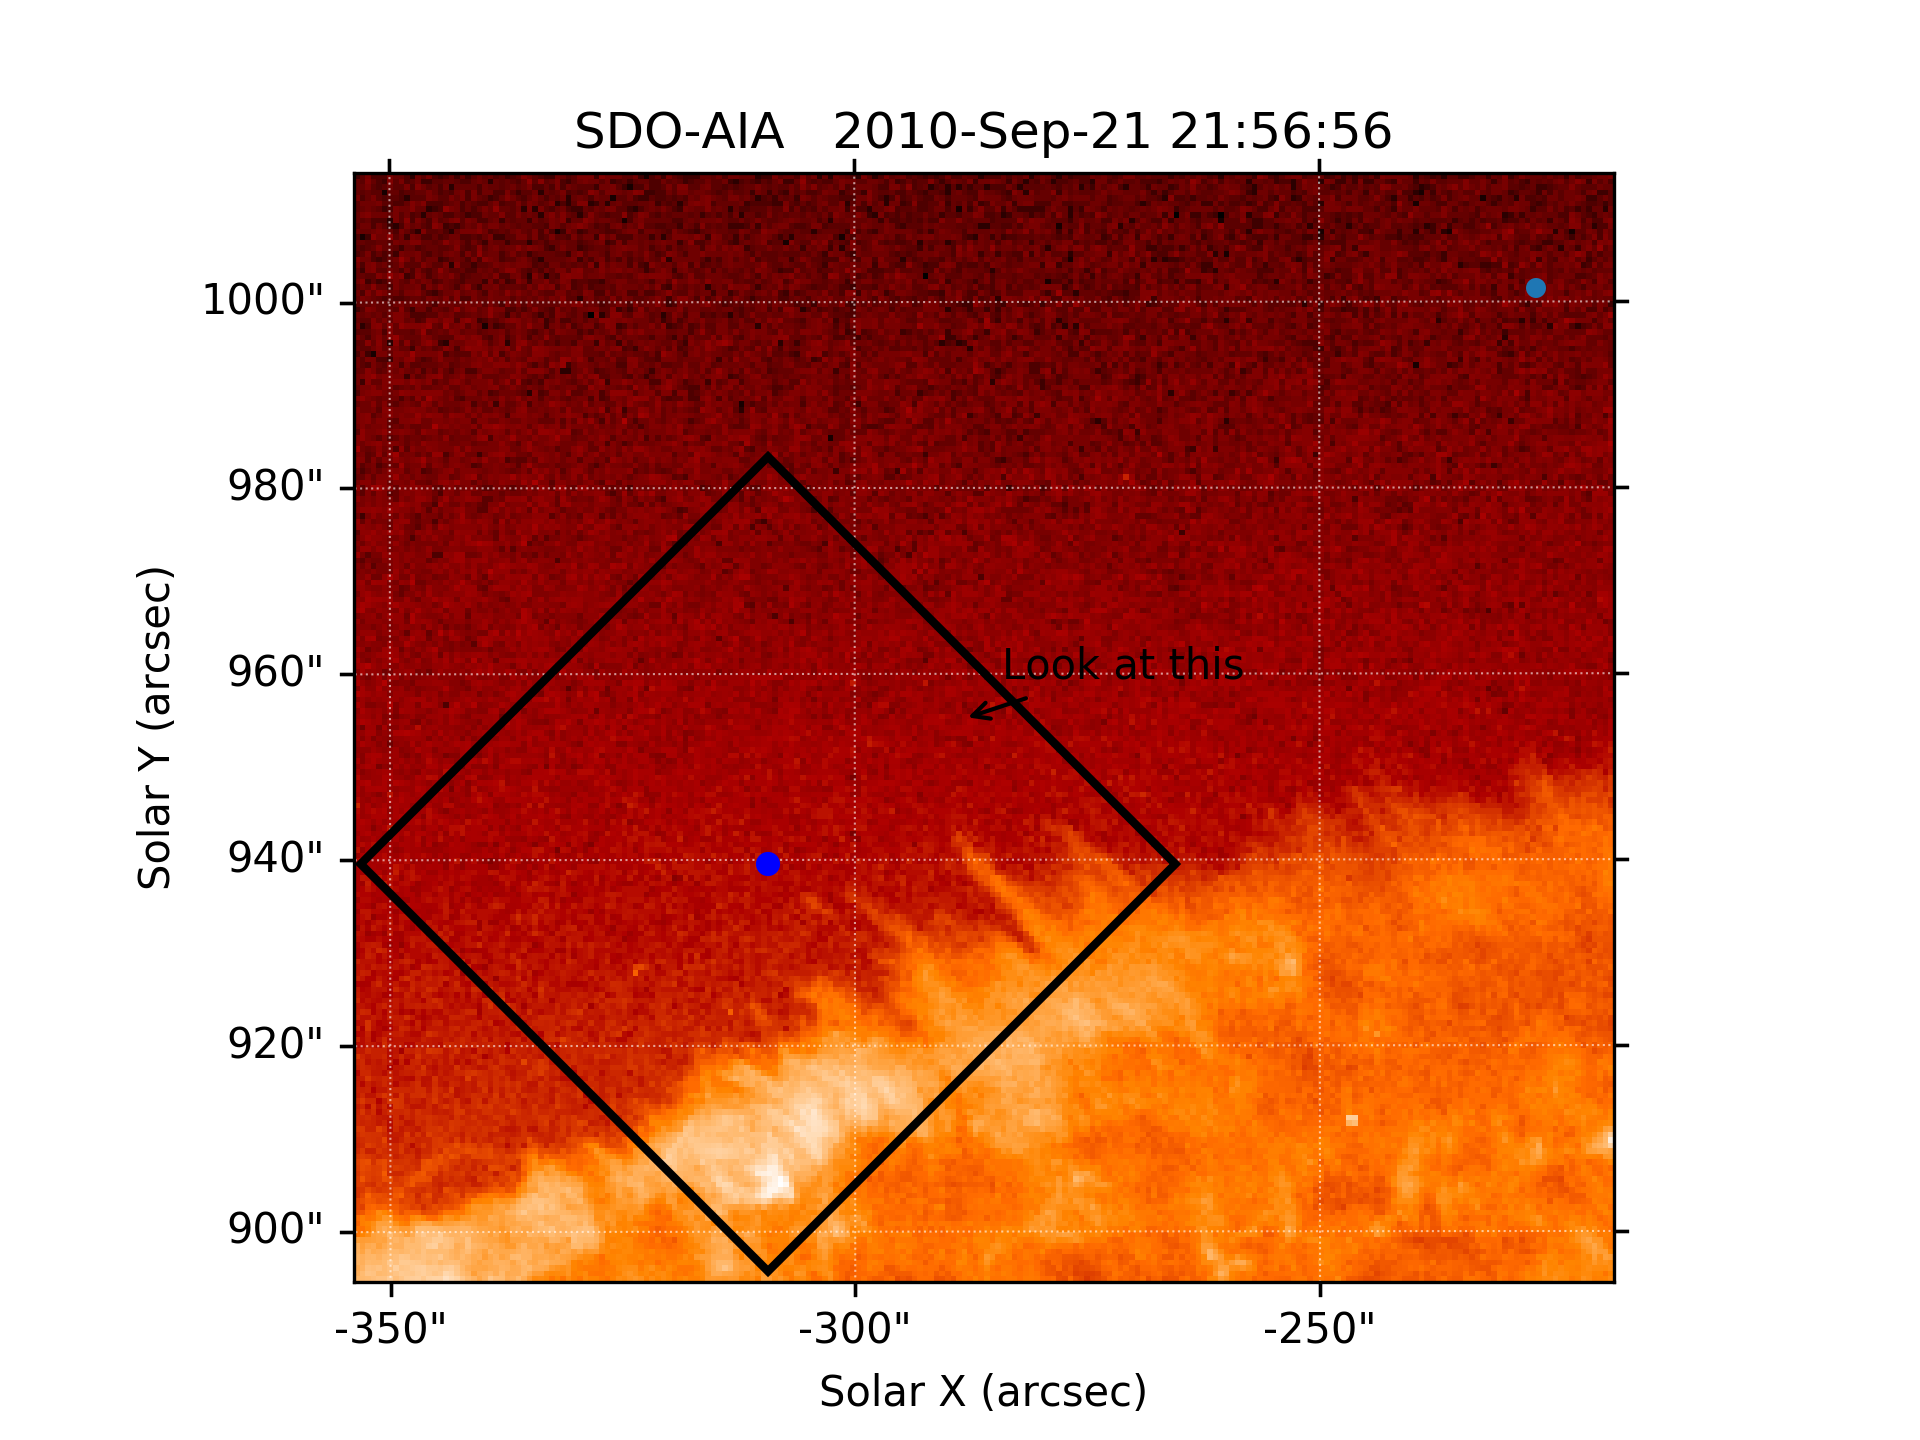
\includegraphics[width=0.4\linewidth]{images/annots.png}
\end{figure}
\end{onlyenv}
\end{frame}


\section{Aggregation}%

\begin{frame}[t]
    \frametitle{Aggregation}

    At present, this program contains only rudimentary methods for aggregating and processing the classified data.

The purpose of data aggregation is take the large number of different classifications made by zooniverse volunteers and attempt to extract a smaller amount of high quality data by doing some sort of “averaging.” Of course, because of the complexity of the data, simply averaging is insufficient. Instead we use a number of clustering algorithms. 
\end{frame}

\begin{frame}{Example}
    \only<1>{
    \begin{figure}[]
        \centering
        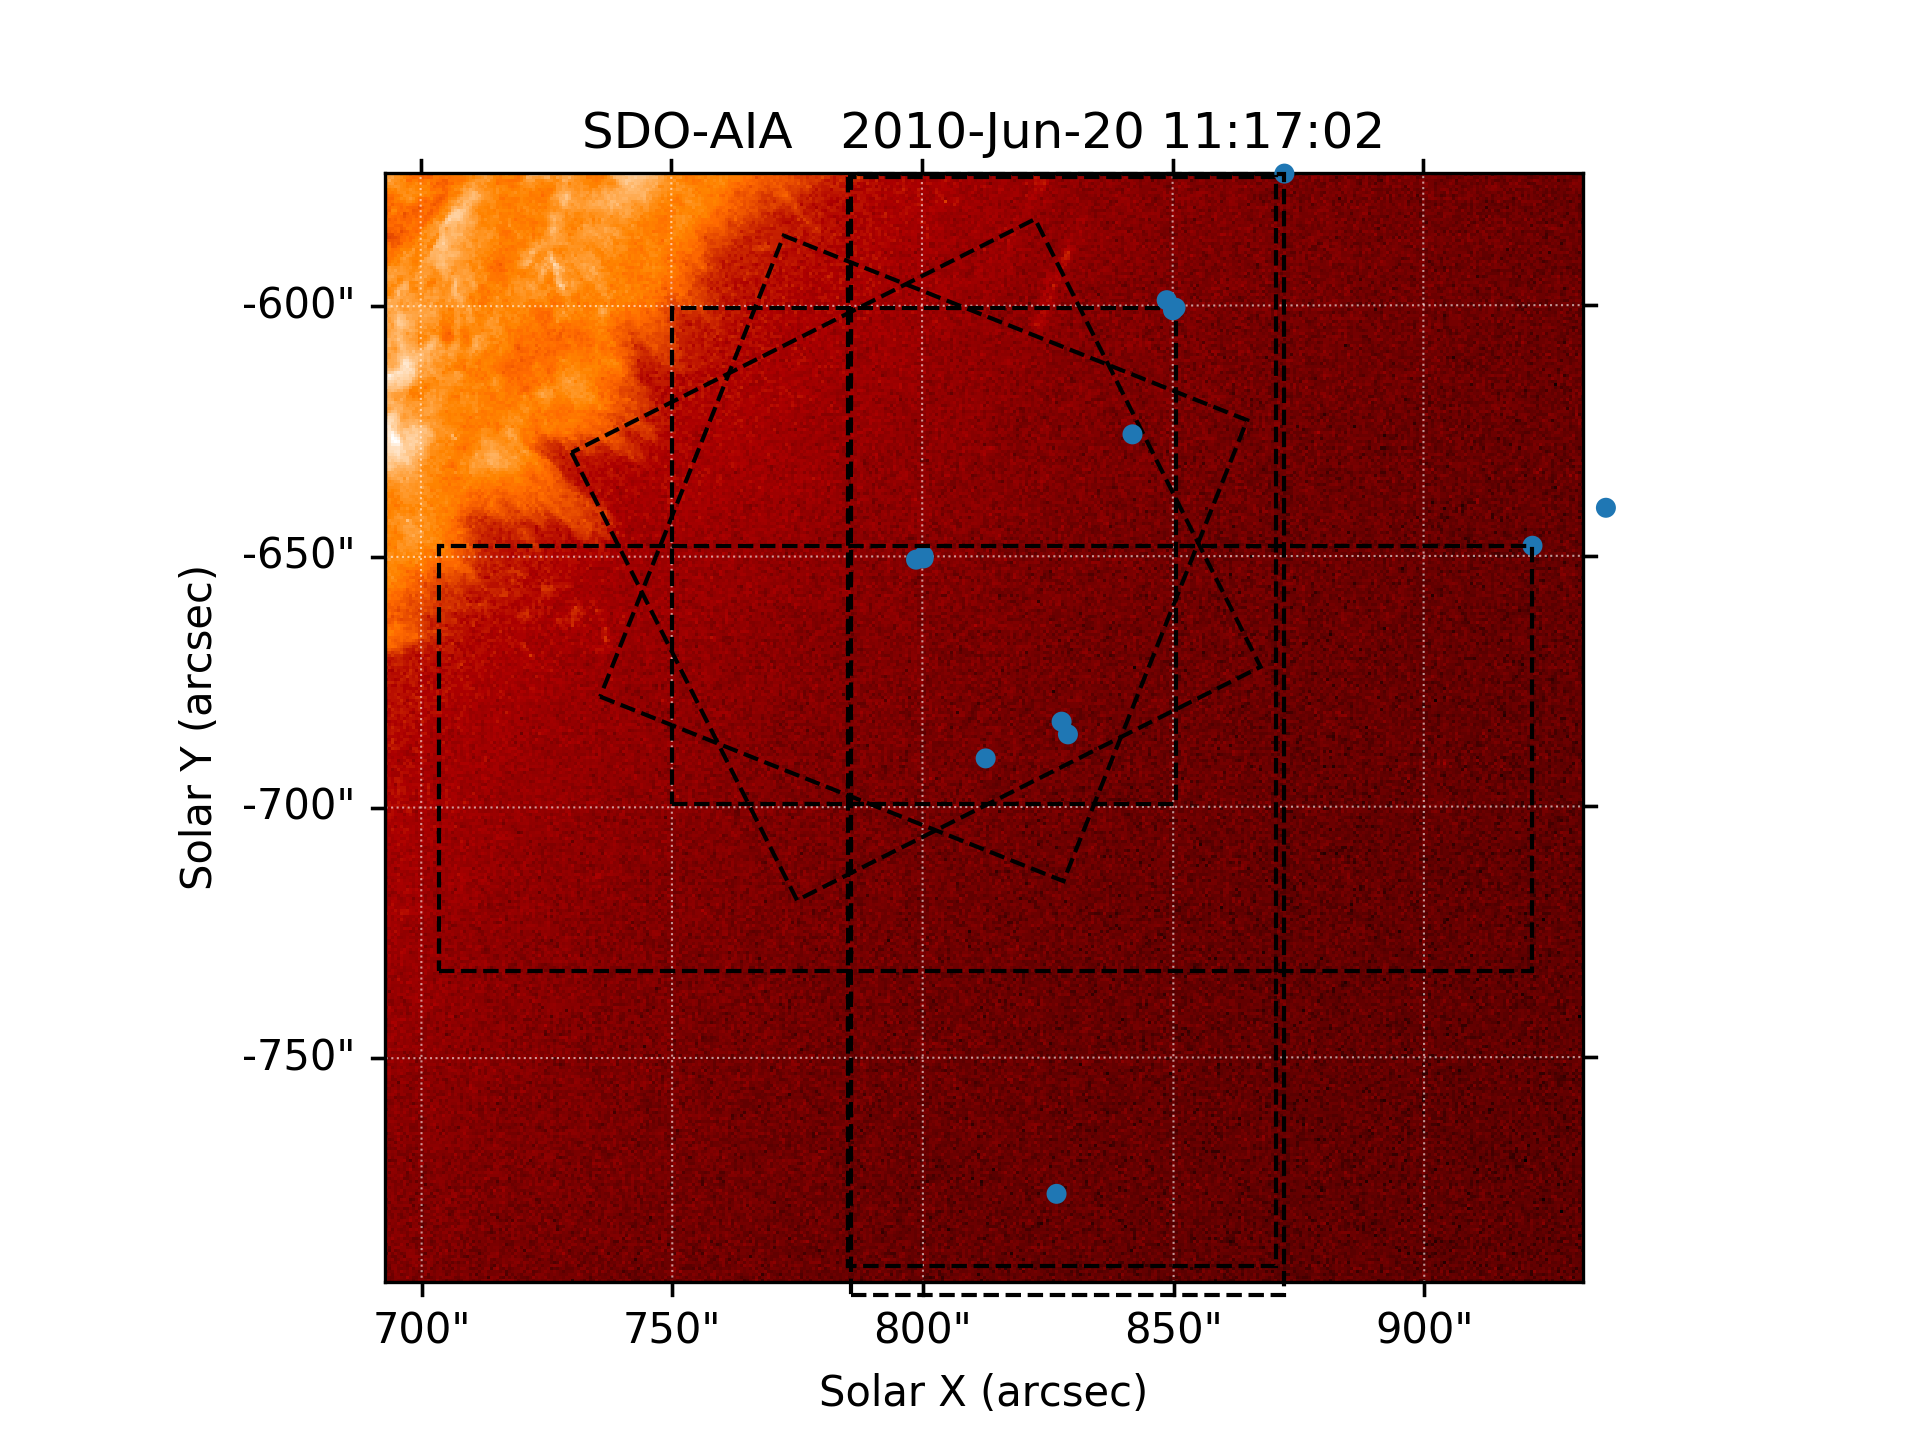
\includegraphics[width=\linewidth]{images/prepreagg.png}
\end{figure}}
    \only<2>{
    \begin{figure}[]
        \centering
        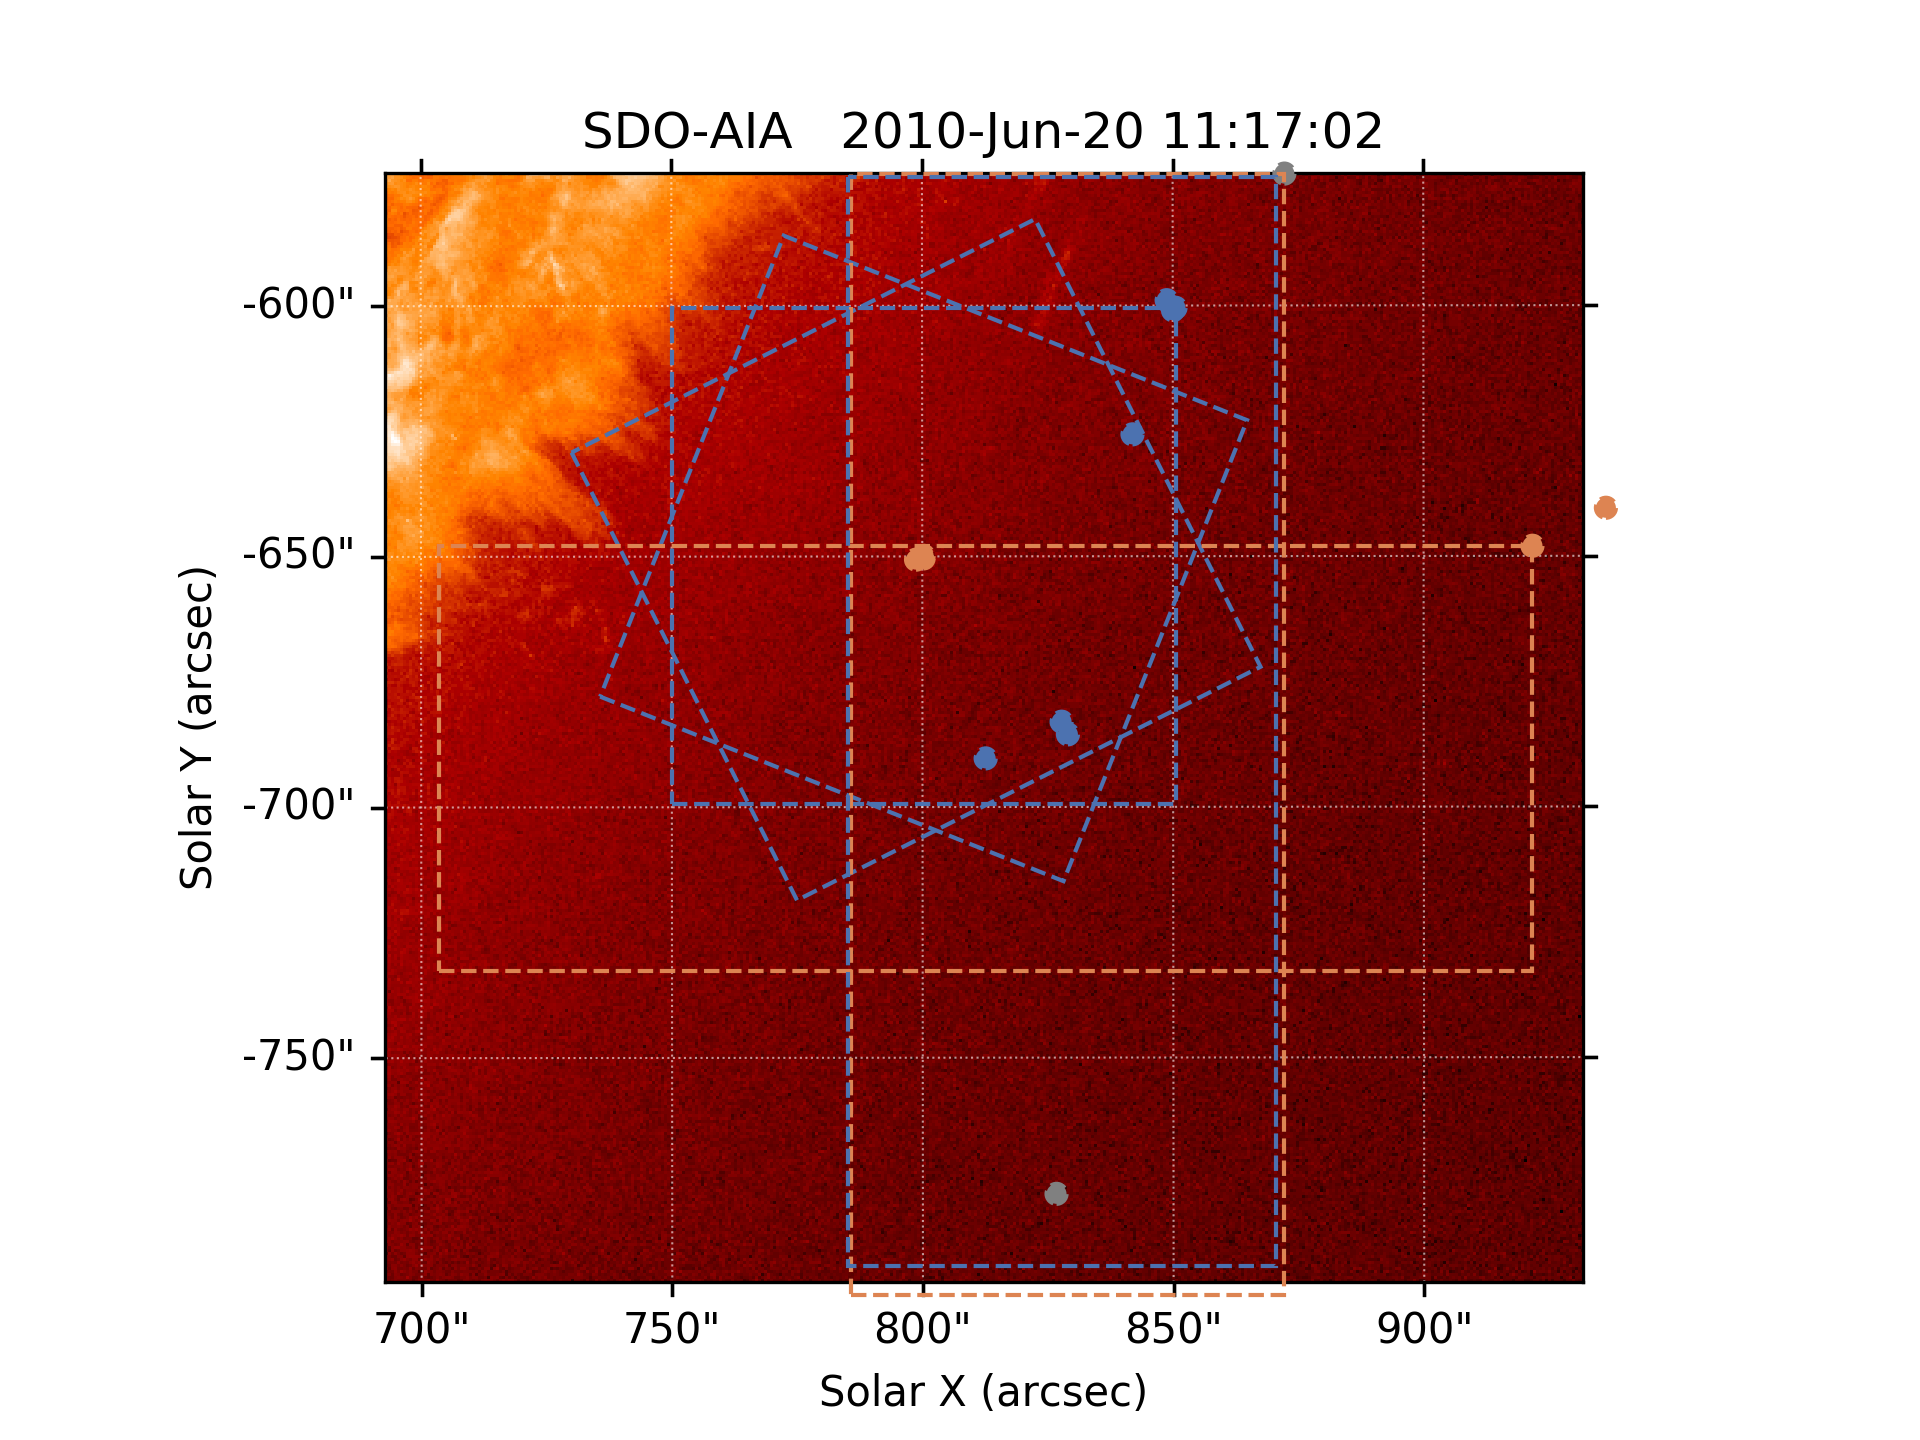
\includegraphics[width=\linewidth]{images/aggpre.png}
\end{figure}}
    \only<3>{
    \begin{figure}[]
        \centering
        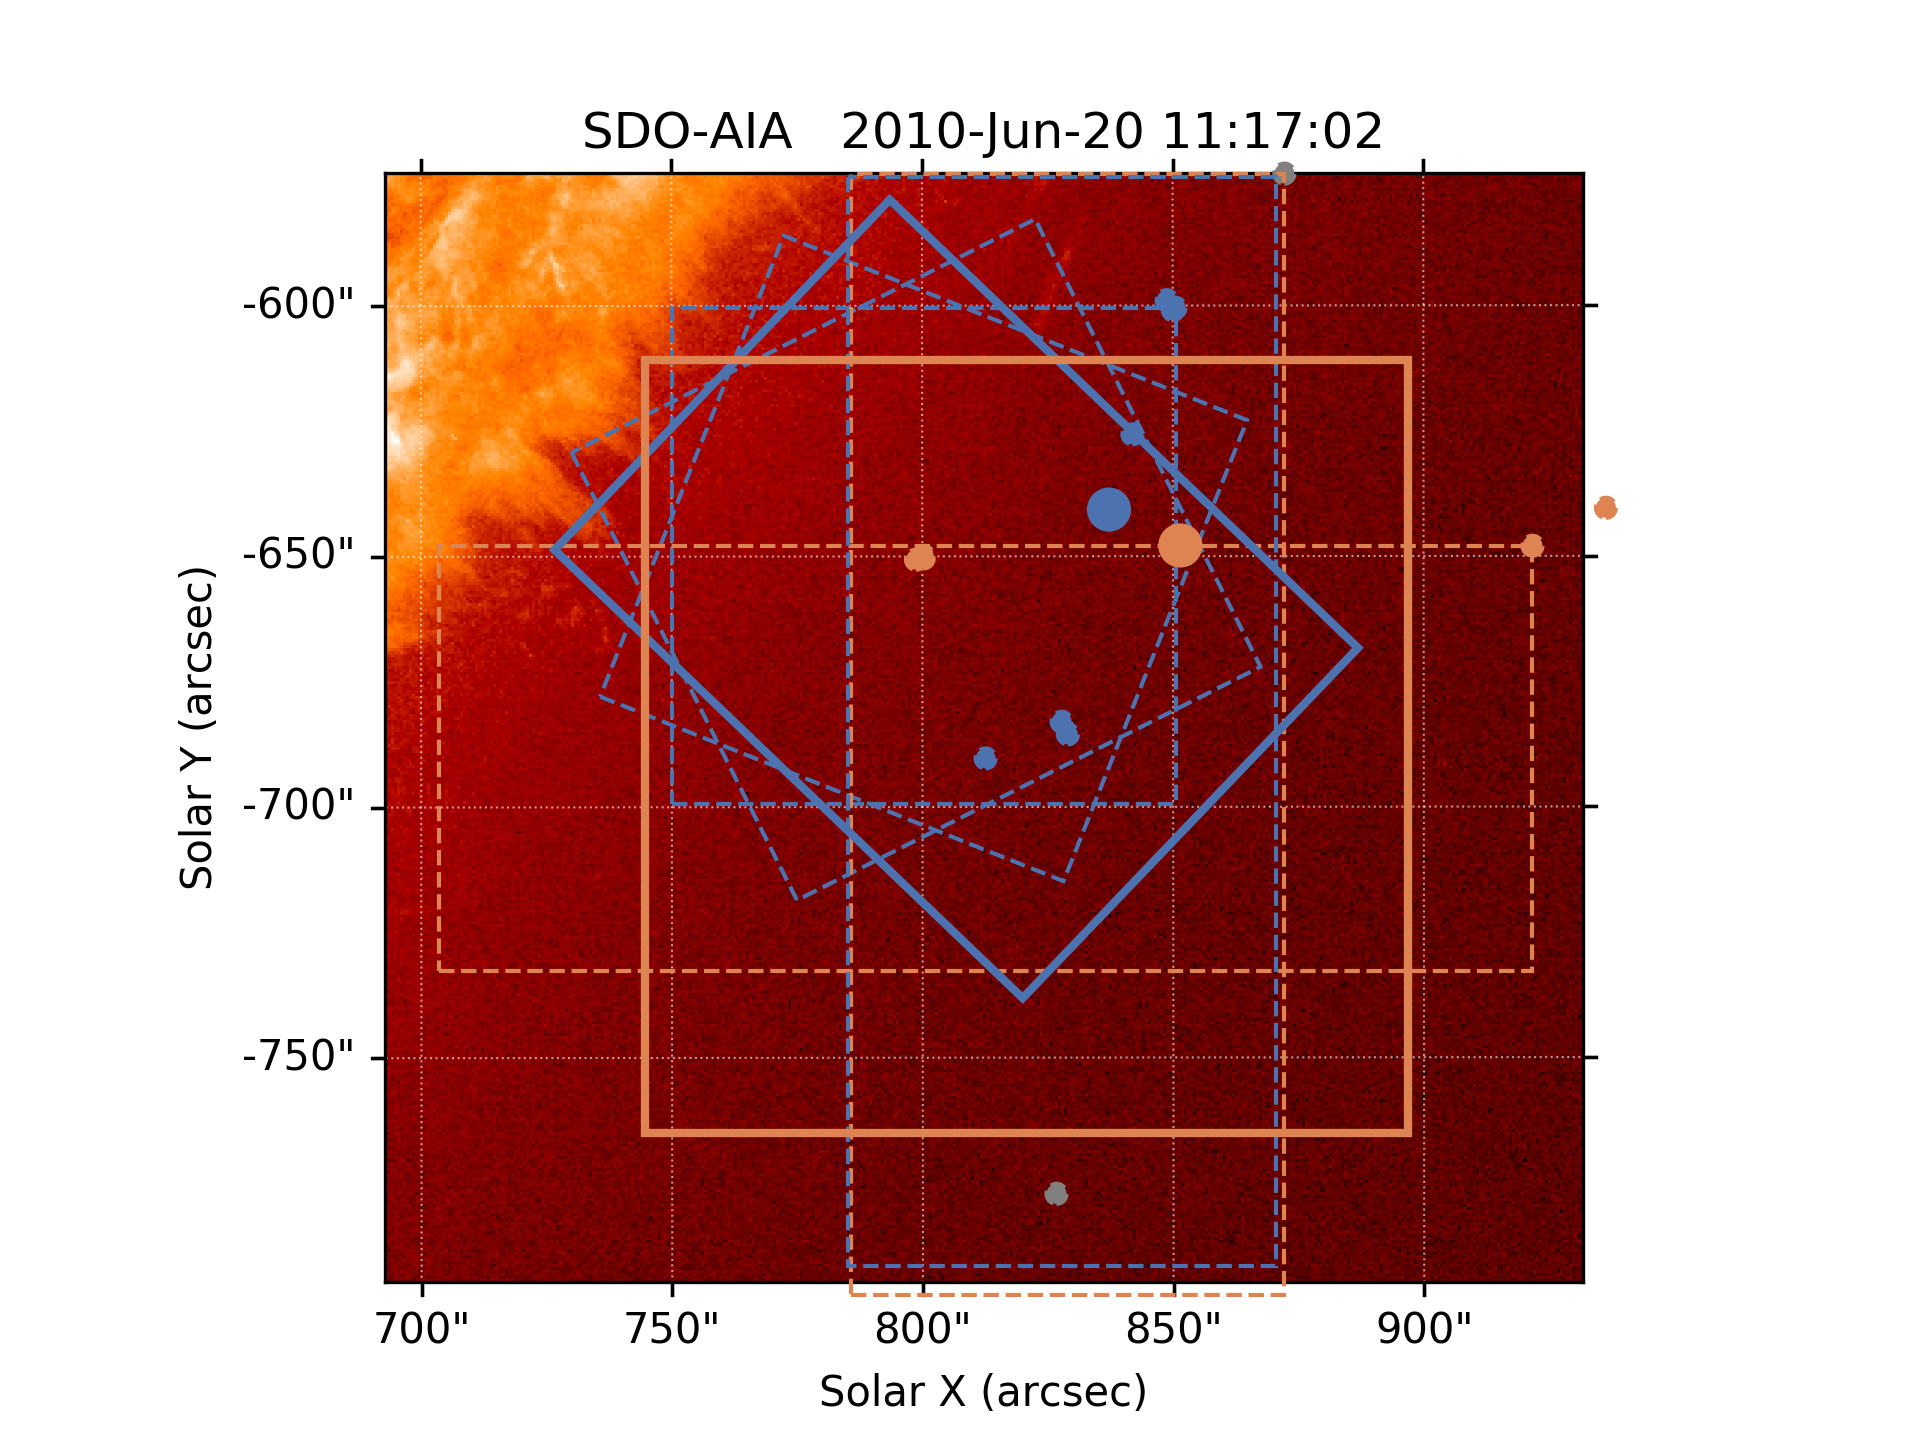
\includegraphics[width=\linewidth]{images/aggexample1.png}
\end{figure}}
\end{frame}


\begin{frame}[t]
    \vspace{2cm}
    \centering\Huge Thank You\\
    \vspace{2cm}
    \centering\Large Questions?
\end{frame}


\end{document}
